\section{IOS-Messungen
\label{section:iosmeasurements}}
Nachfolgend sind die Messungen auf Mobilgeräten mit iOS-Betriebssystem
und daraus gewonnene Erkenntnisse beschrieben.

Gesamthaft wurden 38 Einzelmessungen in 13 Stunden und 20 Minuten durchgeführt.

\subsection{Versuchsdurchführung}
Die im Unterabschnitt~\ref{subsection:plannedexperiments} genannten Messungen
wurden auf insgesamt drei iPhones durchgeführt, welche in der Tabelle 
~\ref{table:measurediosdevices} aufgeführt werden. 

\begin{table}[h!]
	\centering
	\begin{tabular}{|c|c|c|}
		\hline
        \textbf{iPhone Typ} & \textbf{iOS-Version} & \textbf{Besitzer} \\
        \hline
        iPhone 8 & 14.0.1 & Pascale Meier \\
        iPhone X & 14.0.1 & Raphael Jud \\
        iPhone X & 12.3.1 \& 14.0.1 & IFS \\
        \hline
    \end{tabular}
    \caption{Gemessene iOS-Geräte
    \label{table:measurediosdevices}}  
\end{table}

Die zwei Messungen mit dem iPhone X vom IFS und die Messung mit dem iPhone 8 konnten 
komplett durchgeführt werden. 
Das iPhone X von Raphael Jud stand uns nur für fünf Stunden zur Verfügung und wir mussten uns
auf die wichtigsten Messungen beschränken. 
Dazu haben wir uns entschieden, die Langzeitmessungen zu bevorzugen, 
da in diesen Messungen das Verschleiern der MAC-Adressen besser nachvollzogen 
werden kann. 
Weiterhin haben wir uns entschieden, dass im Bedarfsfall die nicht 
durchgeführten Messungen mit dem iPhone X von Raphael Jud zu einem späteren Zeitpunkt 
nachgeholt werden müssen.

Zusätzlich ist uns aufgefallen, dass die Anzahl der bekannten SSID's in iPhones 
vom Gerät selbst verwaltet wird und wir keinen Zugriff auf die bekannten 
Netzwerke haben und diese nicht beeinflussen können.
Eine kurze Internetrecherche hat ergeben, dass ohne Applikationen von 
Drittherstellern diese Einstellung nicht vorgenommen werden kann.
Es gibt weiterhin die Möglichkeit, die Netzwerkeinstellungen auf dem jeweiligen
iPhone über die Geräteeinstellungen zu löschen.
Beide Optionen konnten auf dem iPhone X von Raphael Jud und dem iPhone 8 nicht durchgeführt
werden, da beides Leihgeräte sind und wir keine Geräteeinstellungen verändern
wollen, die sich nicht rückgängig machen lassen.
Somit mussten wir die Messungen mit unterschiedlichen bekannten SSID's 
auch aus der Versuchsdurchführung streichen.

\clearpage 

Eine weitere Einstellung, die auf Android-Geräten vorgenommen werden kann, auf 
iPhones aber nicht existiert, sind die Privacy Settings.
Auf Andriodgeräten kann in den Lokalitätseinstellungen bestimmt werden, 
ob das Gerät Probe-Requests aussendet, obwohl das WLAN ausgeschaltet ist.
IOS erlaubt nur das ein- und ausschalten der Standorteinstellung.
Wir haben den Messplan dahingehend angepasst, dass die Messungen mit iOS jeweils
mit dem Standort anstatt der Privatsphäreeinstellung durchgeführt werden.

\subsection{Ergebnisse}
Mit den im vorherigen Unterabschnitt genannten Einschränkungen konnten die 
folgenden Messergebnisse produziert werden. 

\subsubsection*{Probe-Requests}
In der Tabelle~\ref{table:iosproberesults} ist ersichtlich, wie viele 
Probe-Requests pro Messung aufgezeichnet wurden, wie viele davon in Bursts 
gruppiert waren, die minimale, durchschnittliche und maximale Burstgrösse 
sowie eine Schätzung der nicht aufgezeichneten Frames und die durchschnittliche 
Zwischenankunftszeit zwischen zwei Bursts.

\begin{landscape}
    \begin{table}[h!]
	    \centering
        \begin{tabular}{|c|c|c|c|c|c|c|c|c|}
            \hline
            \textbf{iPhone} & \textbf{iOS Version} & \textbf{Anzahl} & \textbf{Anzahl} & \textbf{min.} & \textbf{avg.} & \textbf{max.} & \textbf{Verpasste} & \textbf{Zwischen-}\\
             & & \textbf{Probes} & \textbf{Bursts} & \textbf{Burstgrösse} & \textbf{Burstgrösse} & \textbf{Burstgrösse} & \textbf{Frames} & \textbf{ankunftszeit}\\
            \hline
            iPhone 8 & iOS 14.0.1 & 1219 & \phantom{0}327 & 1 & 4.372 & 26 & 1196 & 67.02 s \\
            \hline 
            iPhone X - R.J. & iOS 14.0.1 & 1070 & \phantom{0}309 & 1 & 3.849 & 12 & 2382 & 58.27 s \\
            \hline 
            iPhone X - IFS & iOS 12.3.1 & \phantom{0}762 & \phantom{0}193 & 1 & 4.051 & 12 & 1809 & 48.51 s \\
            \hline
            iPhone X - IFS & iOS 14.0.1 & 1784 & \phantom{0}400 & 1 & 4.609 & 18 & 2320 & 36.03 s \\
            \hline
            TOTAL & & 4835 & 1229 & 1 & 4.220 & 26 & 7707 & 52.46 s \\
            \hline
        \end{tabular}
        \caption{Ergebnisse der iOS-Messungen
        \label{table:iosproberesults}}  
    \end{table}
    Die genauen Auswertungen der Messergebnisse finden sich im 
    Anhang~\ref{chapter:appendix:experimentaldata}. 
    Die Daten sind auf dem Repository im Ordner "Experimente" in den jeweiligen Unterordnern
    zu finden.
    
    Nachfolgend sind in den Abbildungen die Graphische Auswertung nach Gesamtzahl 
    (Abbildung~\ref{figure:totaliosmeasurements}) der Messwerte und die Messergebnisse nach Kategorie für 
    die einzelnen iPhone-Geräte (Abbildungen~\ref{figure:iosmeasurementsbycategoryiphone-8-14} 
    bis~\ref{figure:iosmeasurementsbycategoryiphone-x-14}) dargestellt.

    \begin{figure}[h!]
        \centering
        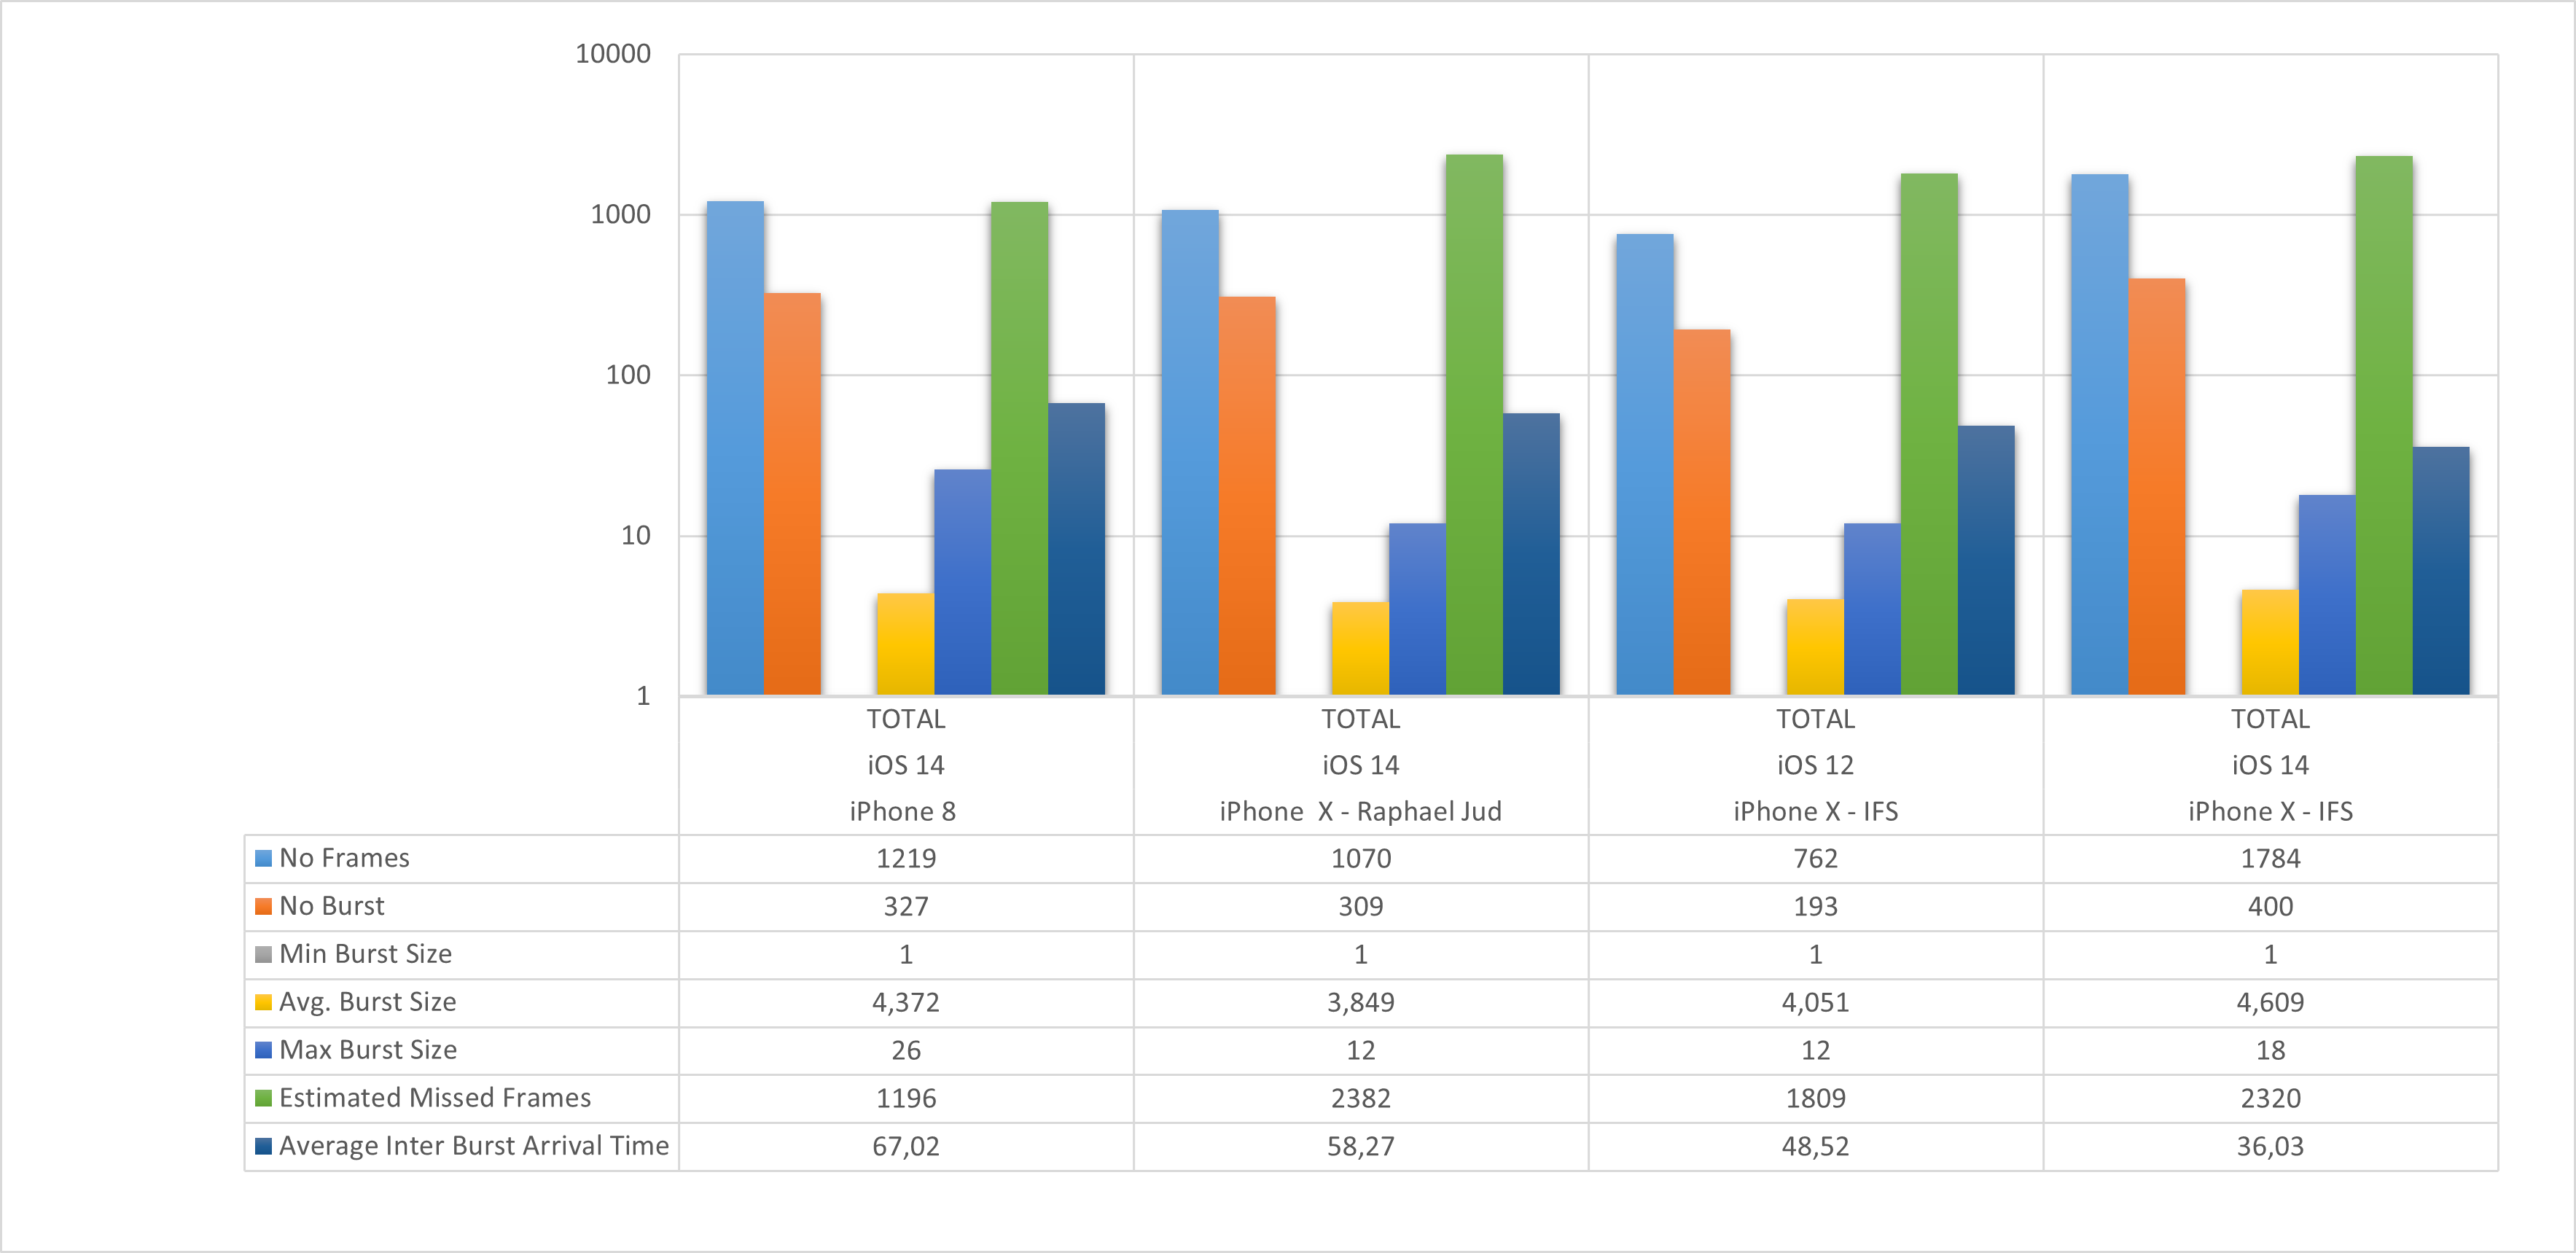
\includegraphics[width=1\linewidth]{Experiments/IOS-Total.png}
        \caption{Gesamtergebnis der iOS-Messungen}
        \label{figure:totaliosmeasurements}
    \end{figure}
\end{landscape}

\begin{figure}[h!]
    \centering
    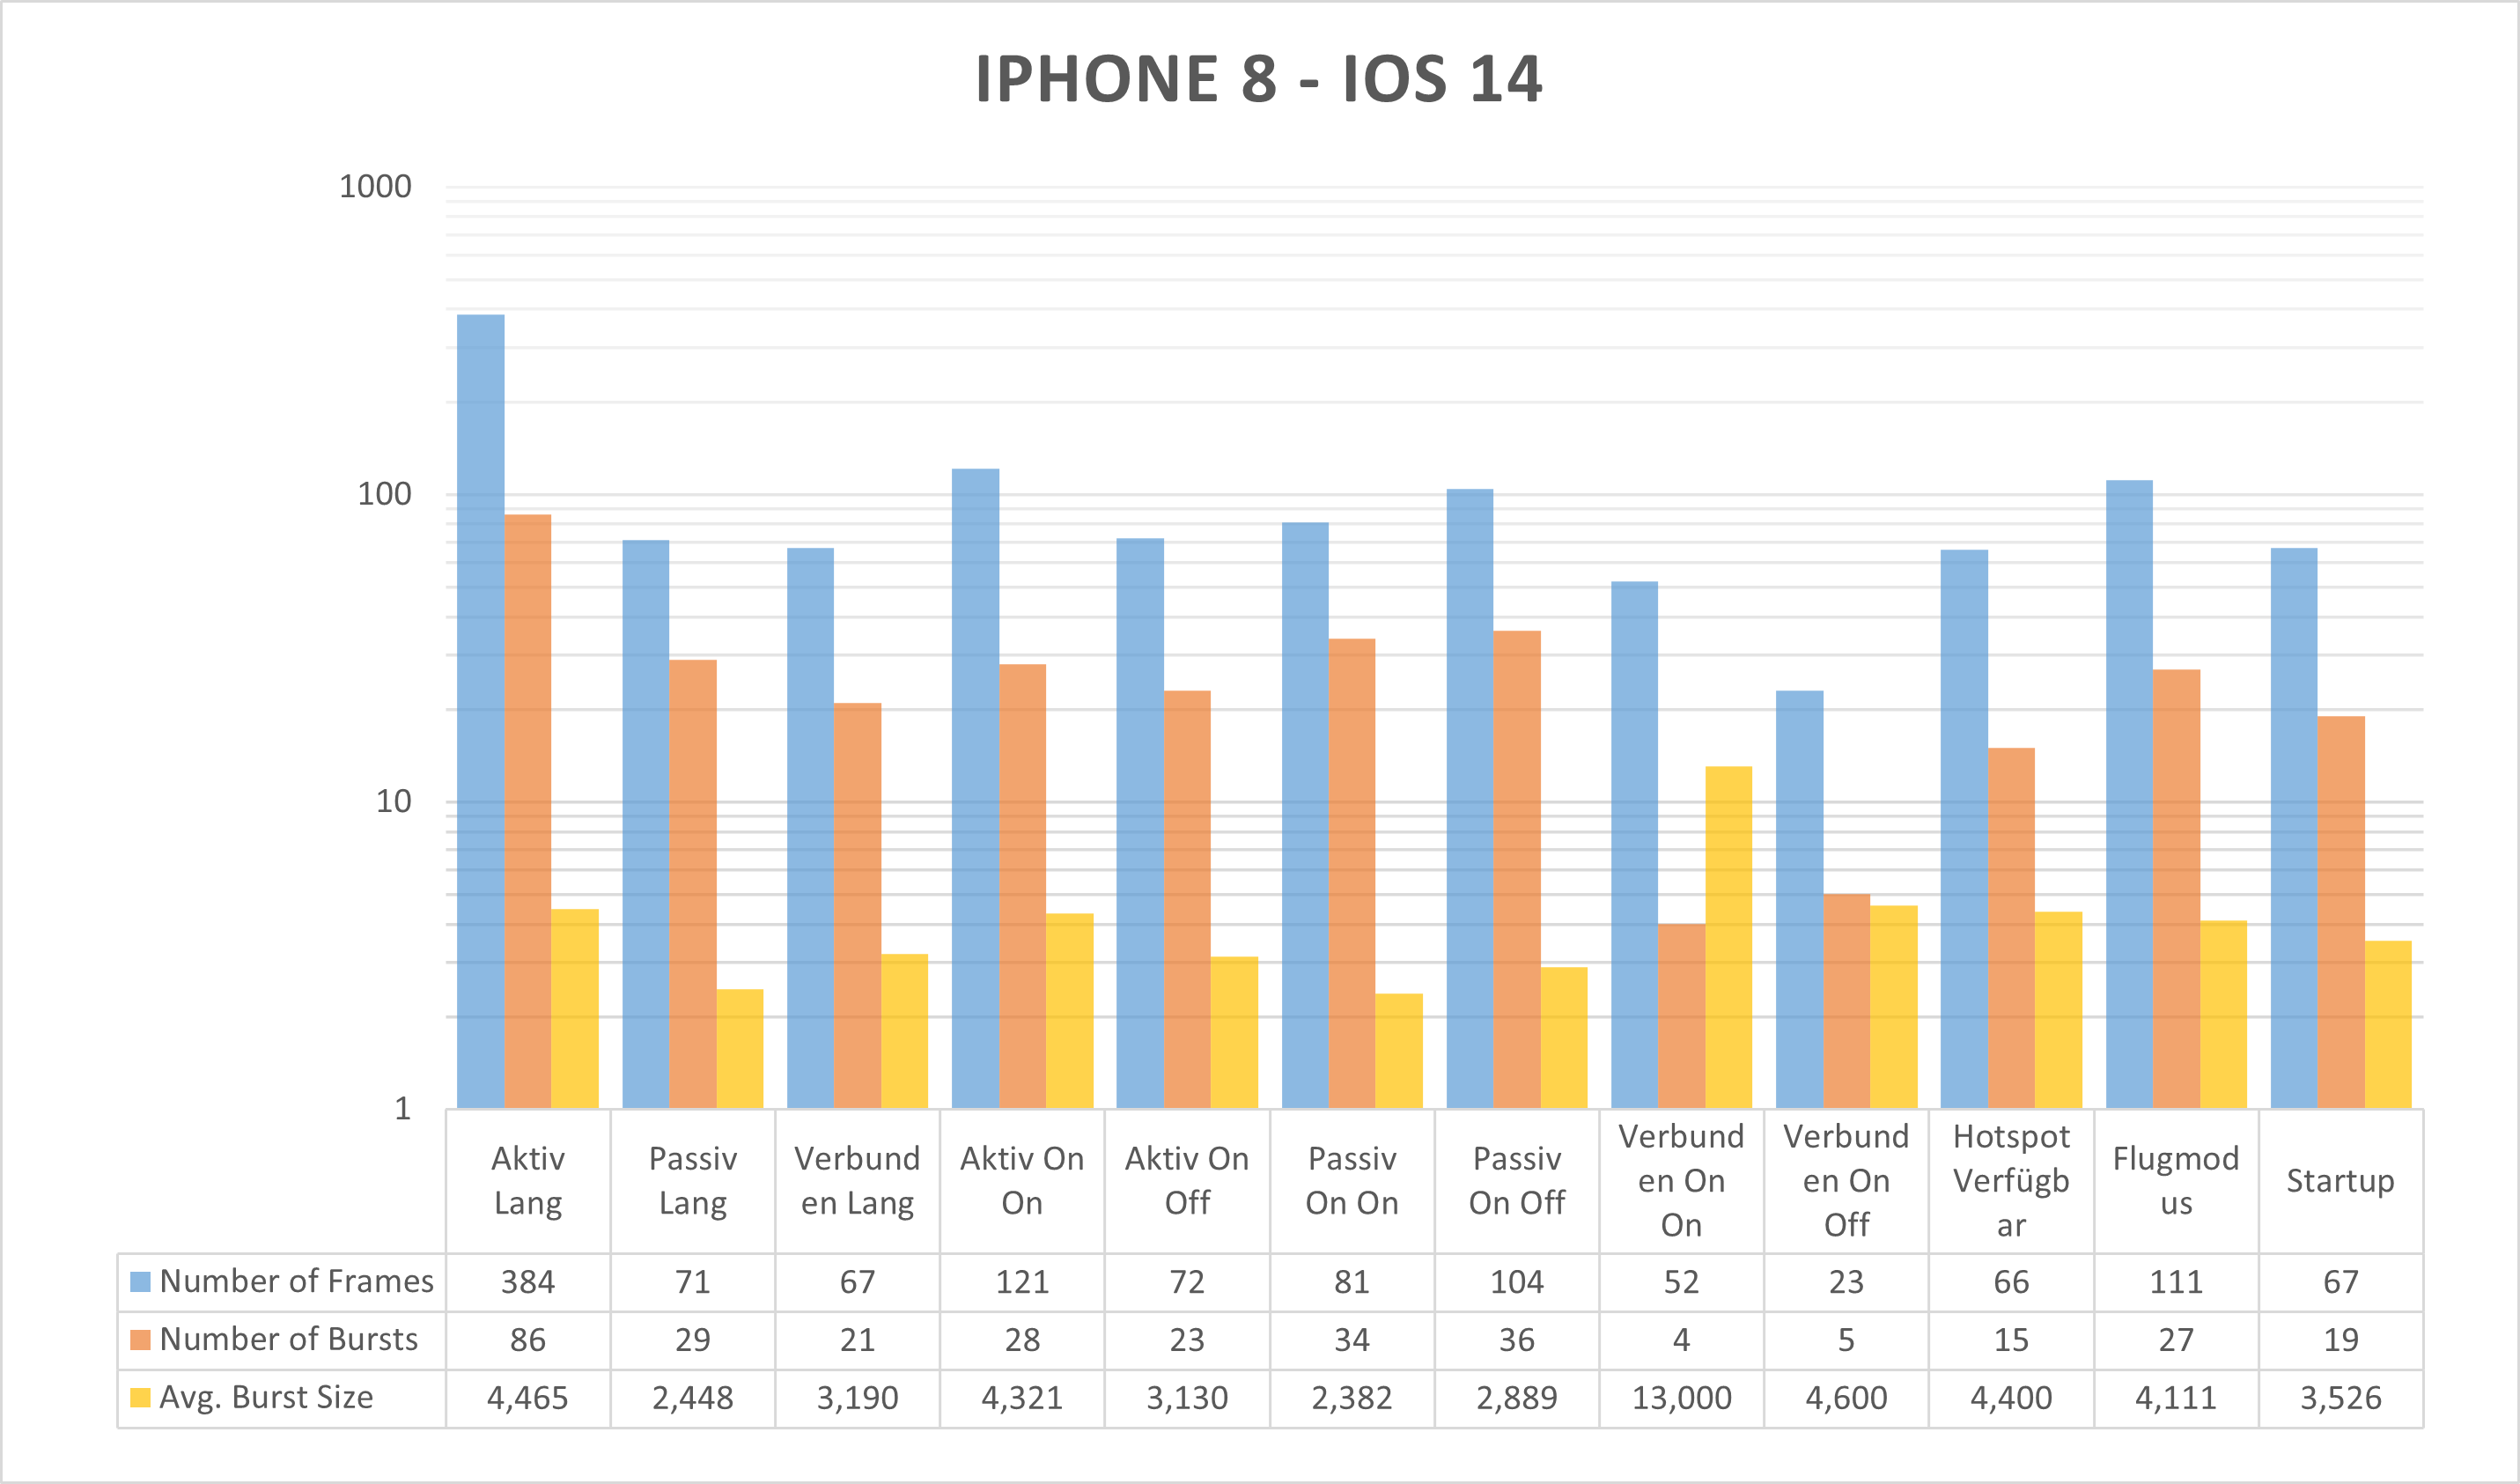
\includegraphics[width=1\linewidth]{Experiments/IPhone8-14.png}
    \caption{Messergebnisse iPhone 8 - iOS 14.0.1}
    \label{figure:iosmeasurementsbycategoryiphone-8-14}
\end{figure}

\begin{figure}[h!]
    \centering
    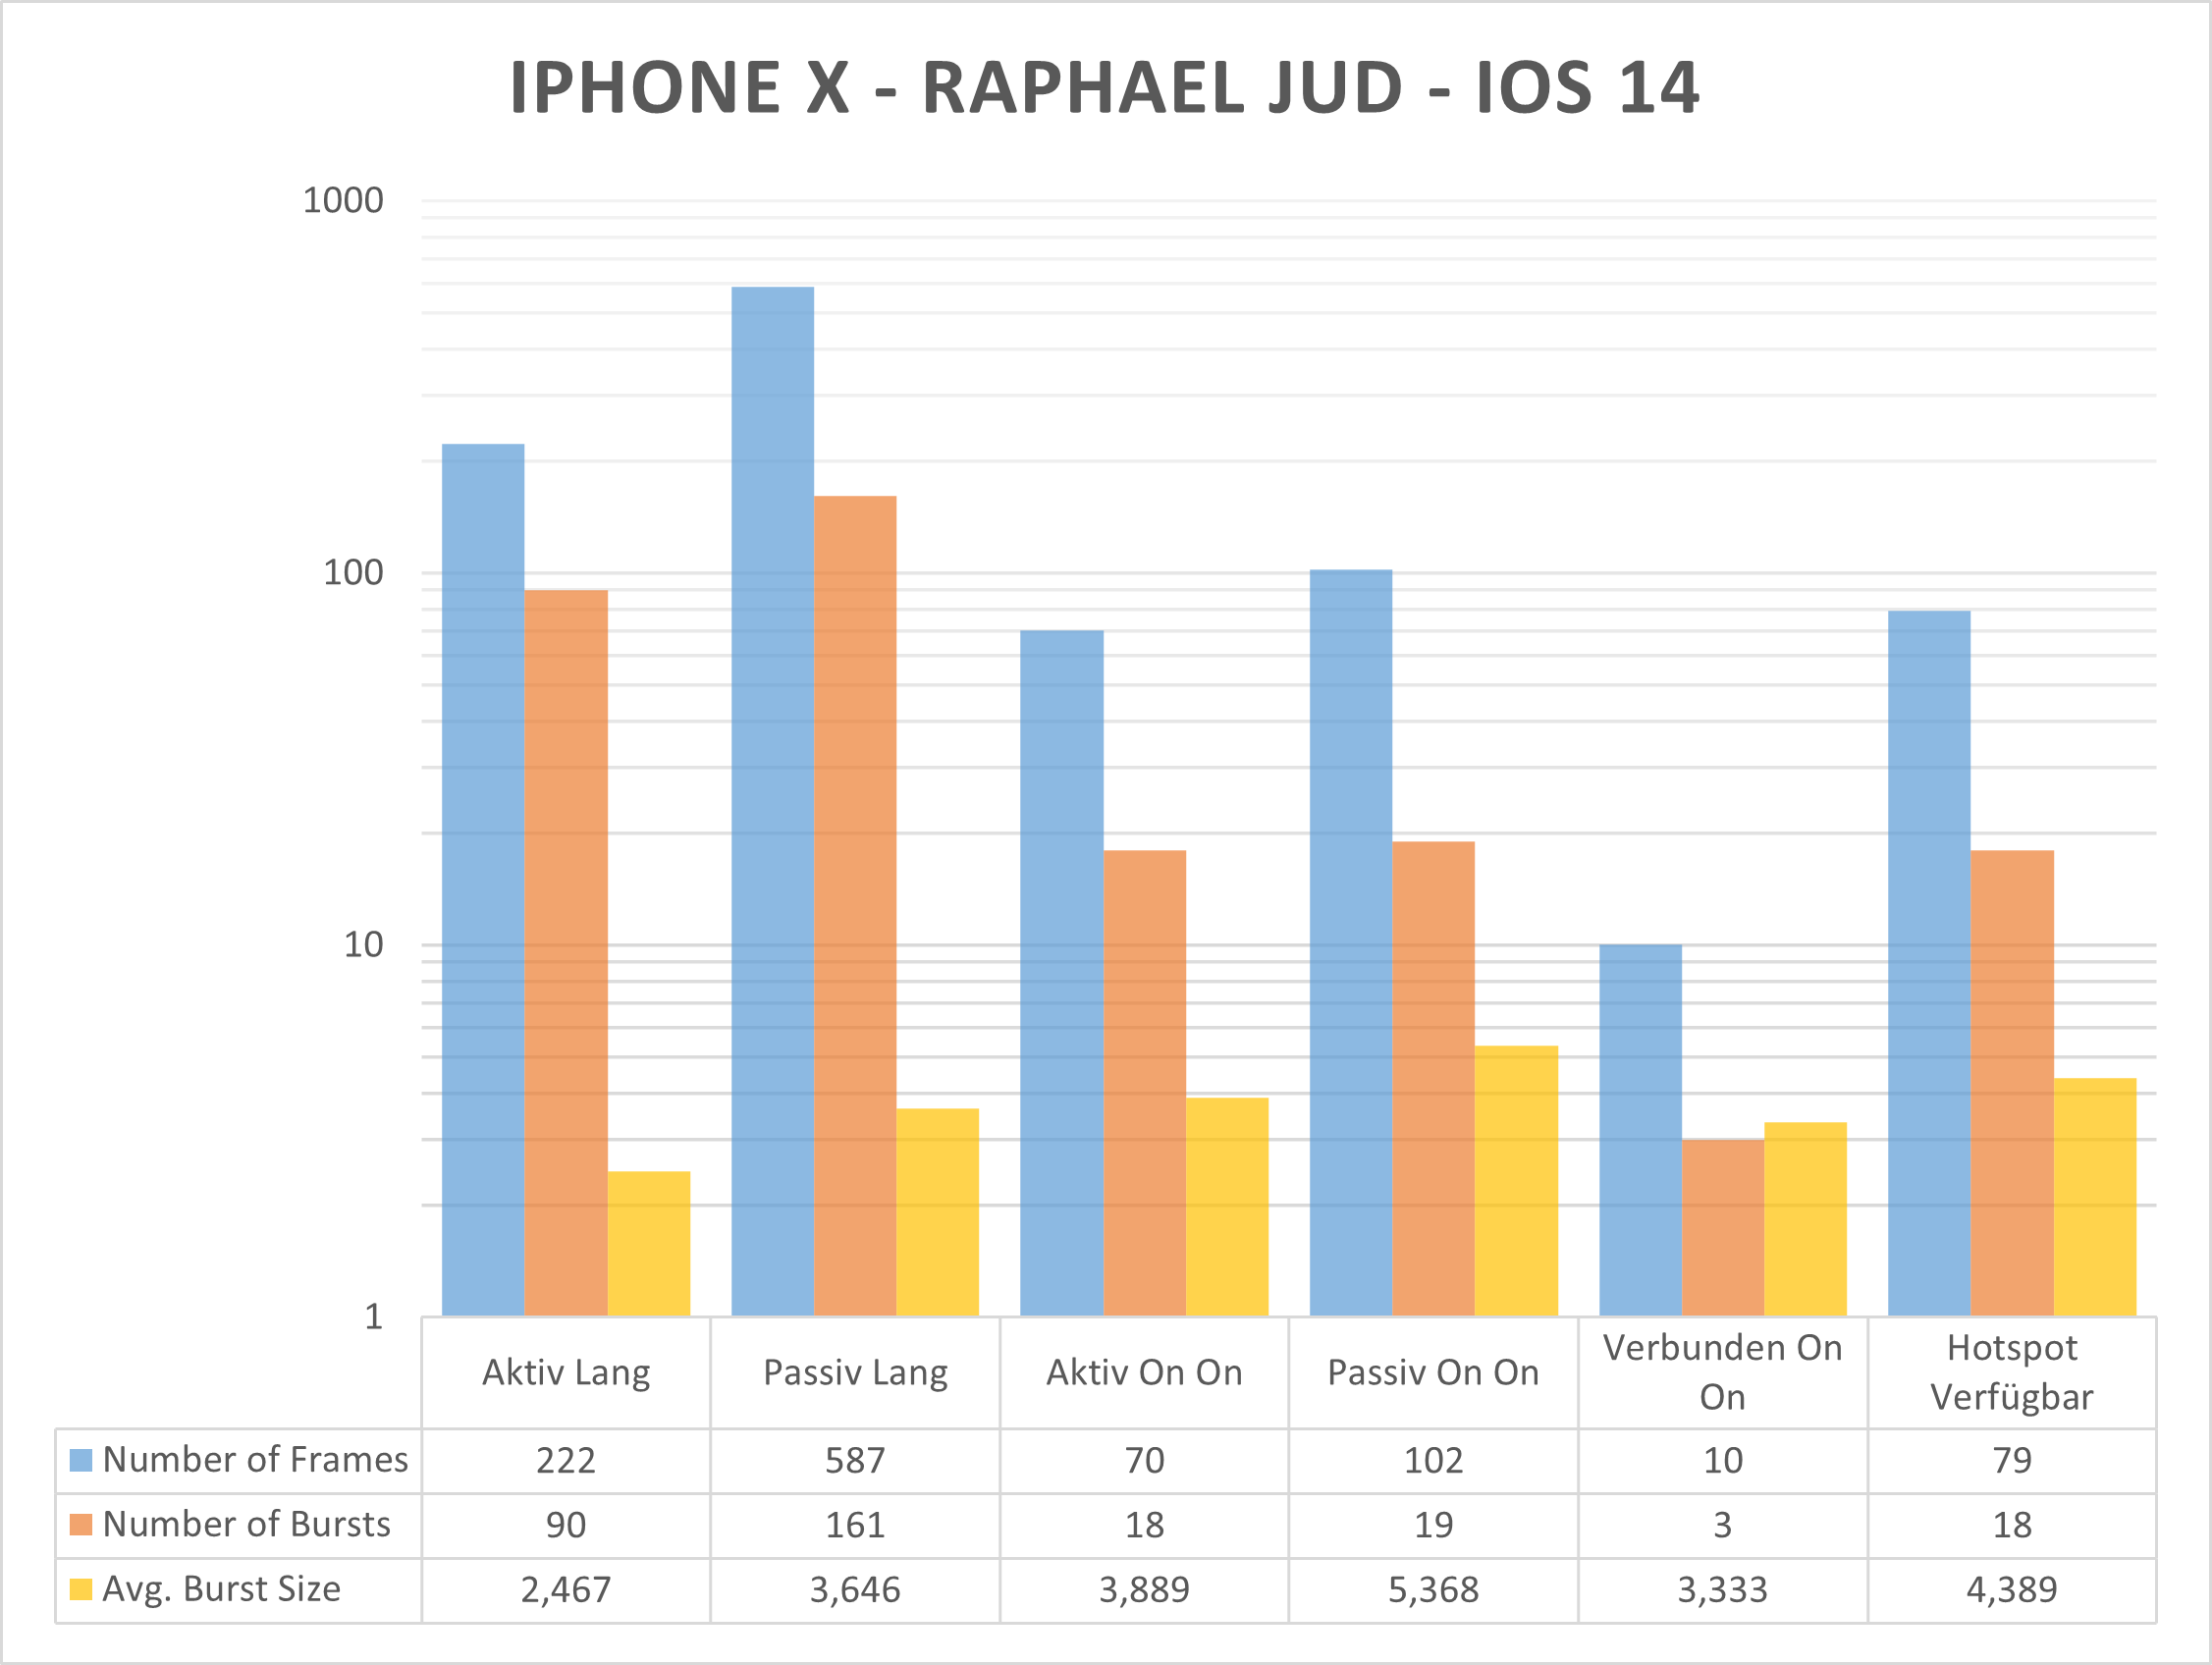
\includegraphics[width=1\linewidth]{Experiments/IPhoneX-RaphaelJud-14.png}
    \caption{Messergebnisse iPhone X - Raphael Jud - iOS 14.0.1}
    \label{figure:iosmeasurementsbycategoryiphone-se-14}
\end{figure}

\begin{figure}[h!]
    \centering
    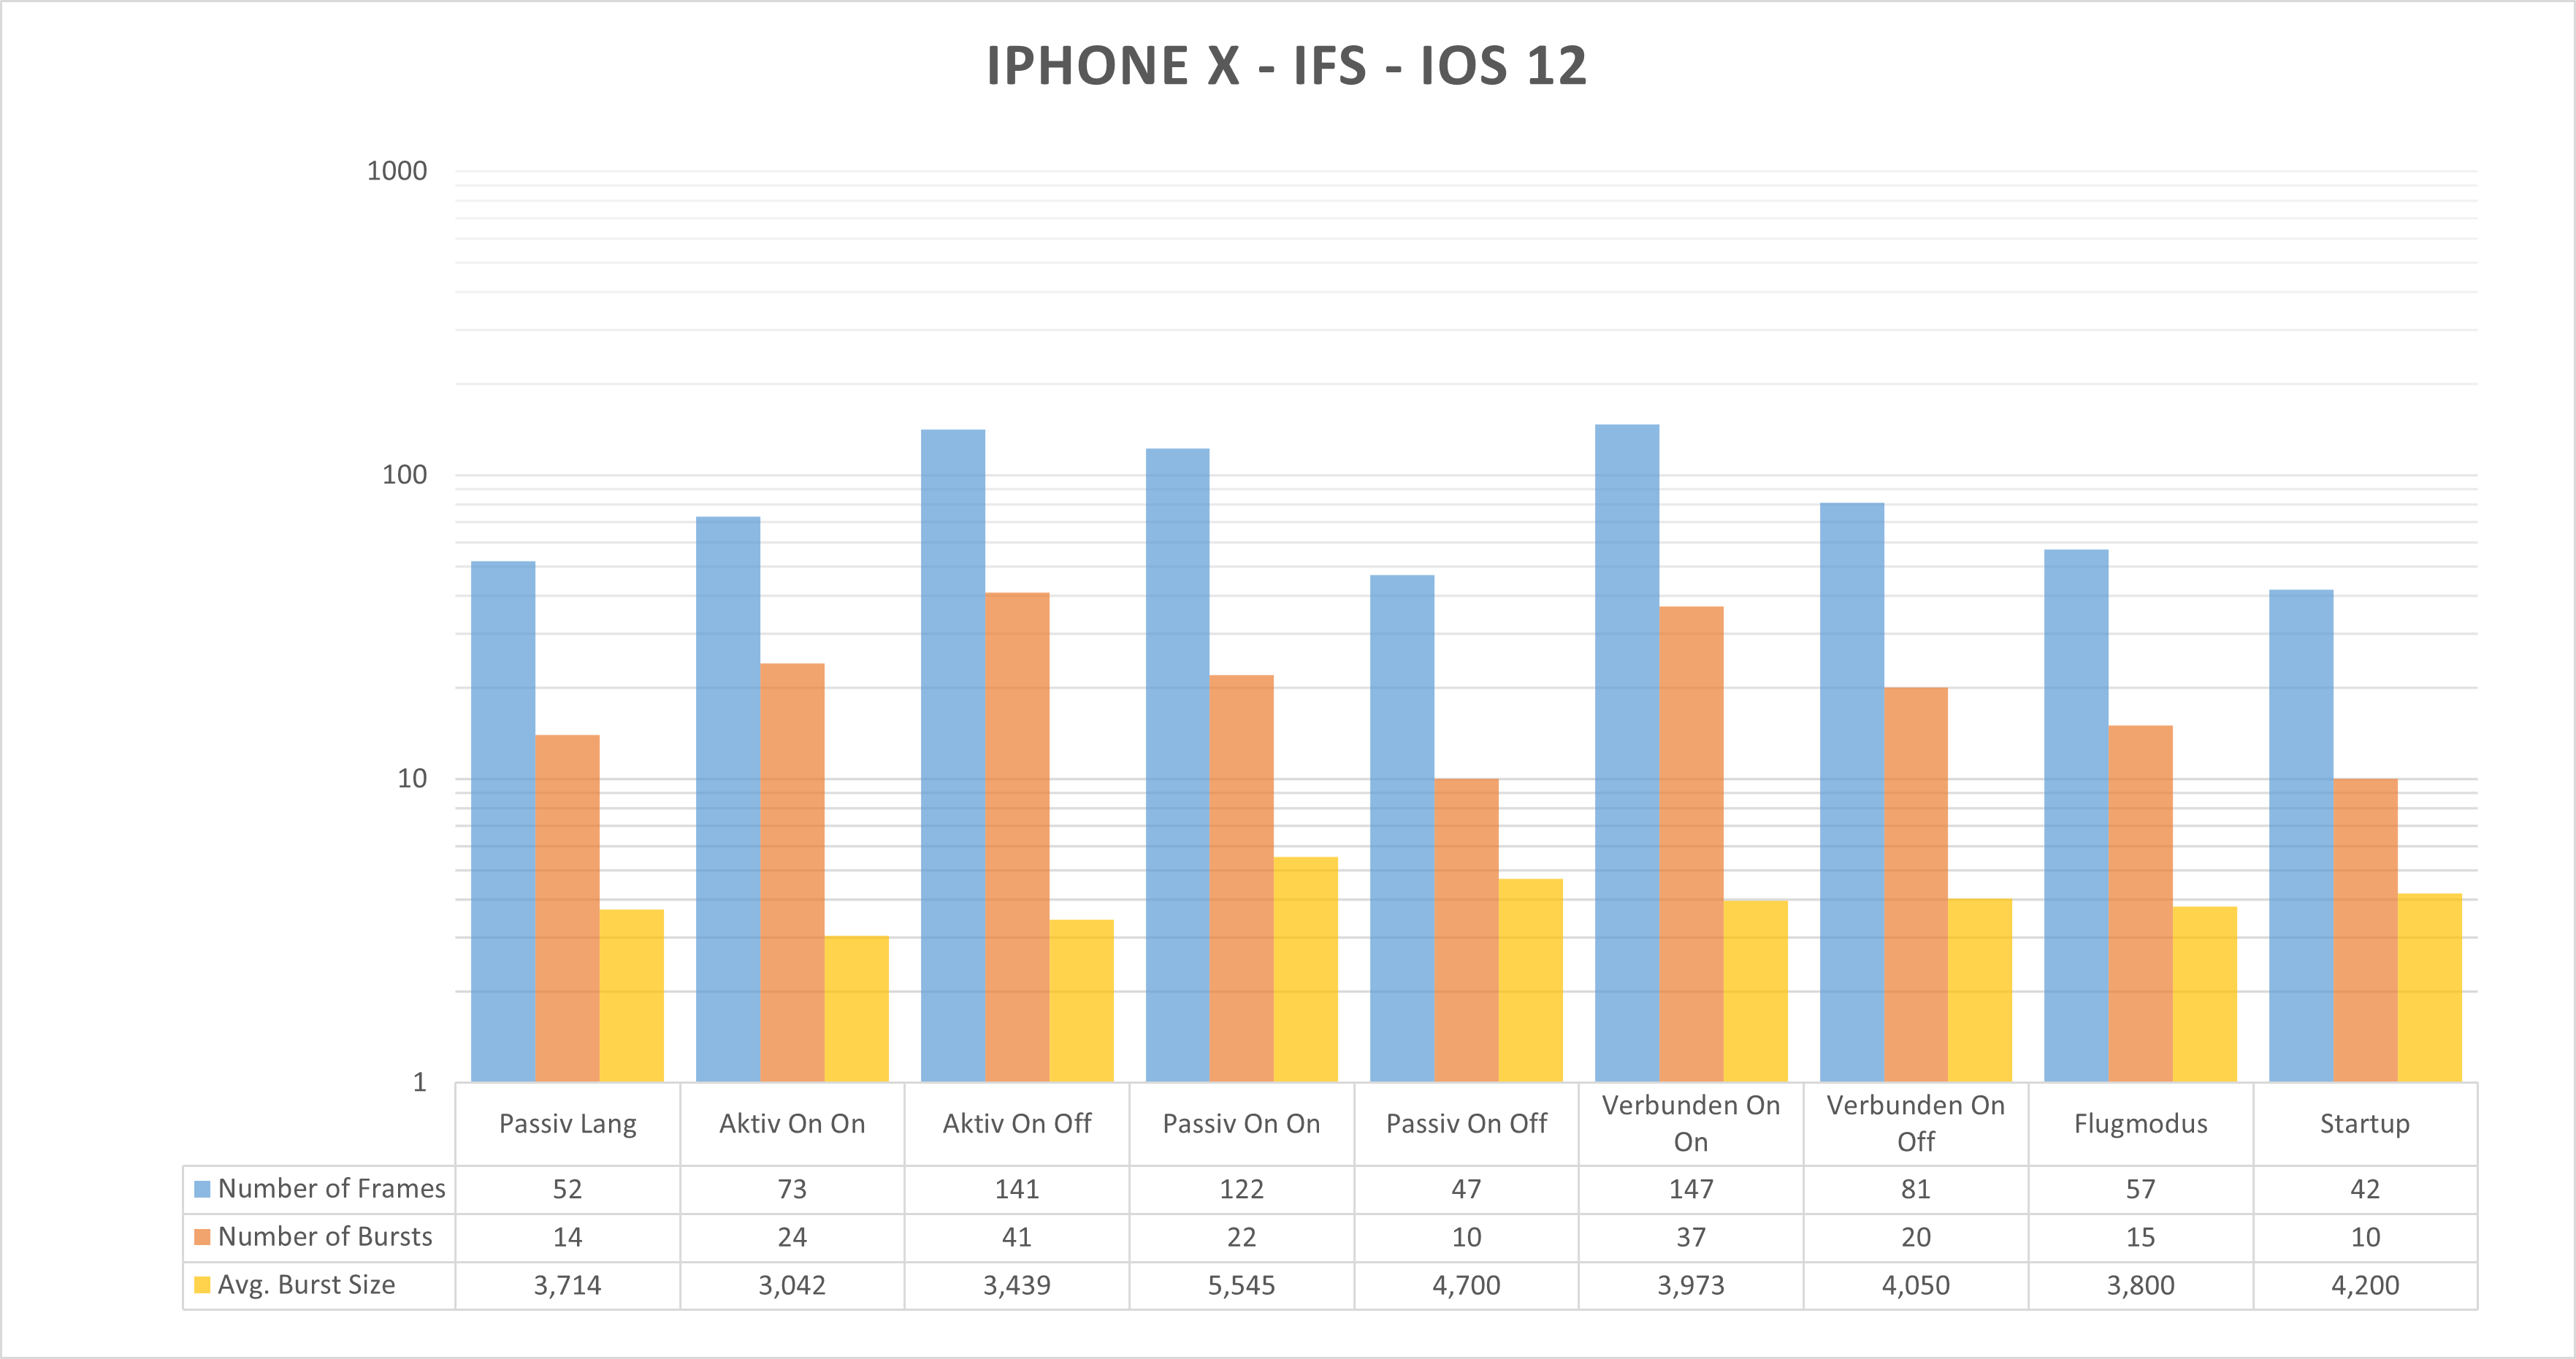
\includegraphics[width=1\linewidth]{Experiments/IPhoneX-IFS-12.png}
    \caption{Messergebnisse iPhone X - IFS - iOS 12.3.1}
    \label{figure:iosmeasurementsbycategoryiphone-x-12}
\end{figure}

\begin{figure}[h!]
    \centering
    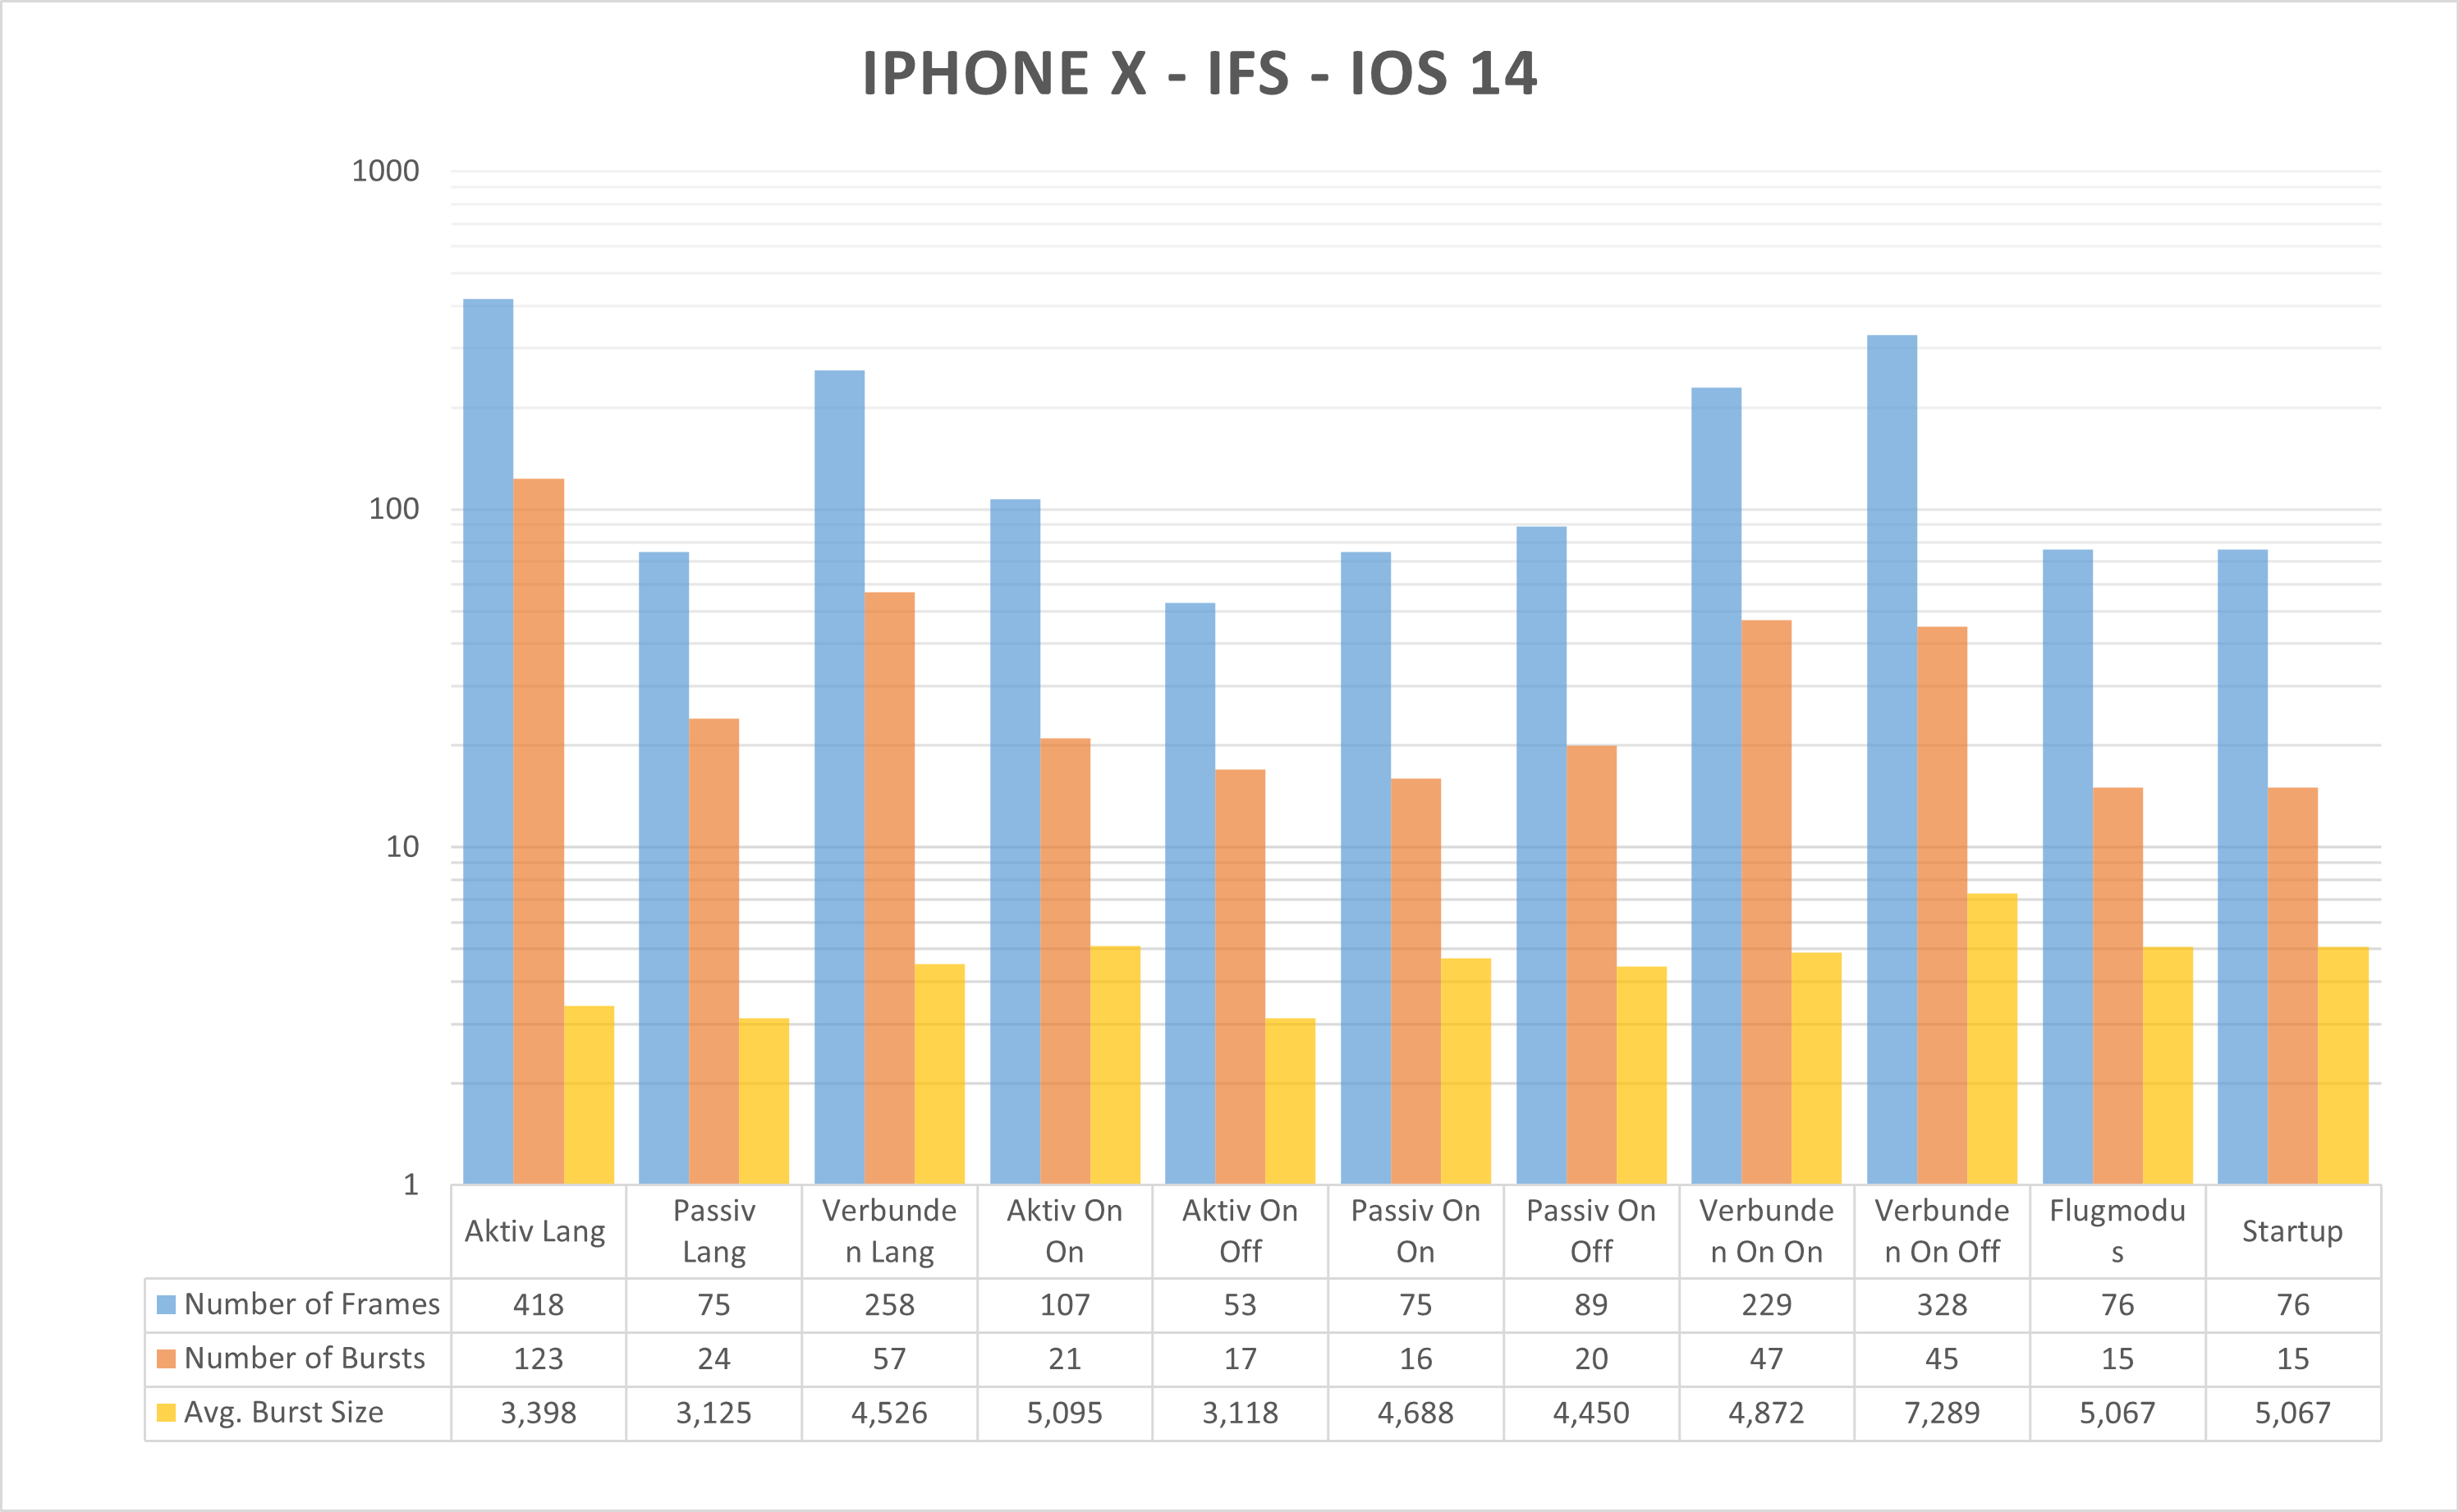
\includegraphics[width=1\linewidth]{Experiments/IPhoneX-IFS-14.png}
    \caption{Messergebnisse iPhone X - IFS - iOS 14.0.1}
    \label{figure:iosmeasurementsbycategoryiphone-x-14}
\end{figure}

\clearpage

\subsubsection*{Erkenntnisse aus den iOS-Messungen}
In total $4835$ aufgezeichneten Probe-Requests sind im Schnitt jeweils $4.22$ 
Frames pro Burst mit einer durchschnittlichen Zwischenankunftszeit von $52.46 s$
gemessen worden. Die Bursts haben eine Grösse zwischen einem und 26 Frames.

Anhand der Sequenznummern innerhalb eines Bursts kann abgeschätzt werden, wie 
viele Frames im Burst nicht aufgezeichnet (verpasst) werden.
In den iOS-Messungen wurden schätzungsweise $7707$ Frames verpasst.
Eine mögliche Erklärung für die hohe Anzahl verpasster Frames ist, dass
iPhones zwischen einzelnen Frames den Kanal wechseln bzw. Probe-Requests auf 
wechselnden Kanälen aussenden, anstatt die Probes für einen Kanal zu gruppieren.

Bei genauerer Betrachtung der pcap oder JSON-Dateien zu den einzelnen Messungen
fällt auf, dass iPhones IE-Felder gemäss den Tabellen~\ref{table:ioscommoniefields}, 
\ref{table:iosuncommoniefields} und~\ref{table:iosvendorspecificiefields} 
beinhalten.

\begin{table}[h!]
    \centering
    \begin{tabular}{|c|c|c|c|c|}
        \hline
        \textbf{Tag-NR} & \textbf{0} & \textbf{1} & \textbf{50} & \textbf{3} \\
        \textbf{Tag-Name} & \textbf{SSID} & \textbf{Supported Rates} & \textbf{Ex. Supp. Rates} & \textbf{DS Params Set} \\
        \hline 
        Geräte & alle & alle & alle & alle \\
        \hline
    \end{tabular}
    \caption{IE-Felder, die in allen Messungen vorkommen
    \label{table:ioscommoniefields}}  
\end{table}

\begin{table}[h!]
    \centering
    \begin{tabular}{|c|c|c|c|}
        \hline
        \textbf{Tag-NR} & \textbf{45} & \textbf{127} & \textbf{107} \\
        \textbf{Tag-Name} & \textbf{HT Capabilities} & \textbf{Extended Capabilities} & \textbf{Interworking} \\
        \hline 
        Phones  & alle & alle & alle \\
        \hline
    \end{tabular}
    \caption{IE-Felder der einzelnen iPhones
    \label{table:iosuncommoniefields}}  
\end{table}

Es wird davon ausgegangen, dass die IE-Felder mit den Nummern 0, 1, 50, 3, 45 
und 127 in allen iOS-Geräten verwendet werden. 
Der Interworking Tab mit der Tagnummer 107 wird in verschiedenen Messungen 
mitgesendet, es kann aber aus den Ergebnissen keine Regelmässigkeit herausgelesen
werden, nach welchen Voraussetzungen der Tag verwendet wird.

\clearpage 

\begin{table}[h!]
    \centering
    \begin{tabular}{|c|c|c|c|}
        \hline
        &  \textbf{Apple}  & \textbf{Microsoft Corp.} & \textbf{Broadcom} \\
        \hline 
        iPhone 8 & x  &  & \\
        iPhone X - Raphael Jud - 14 & & & \\
        iPhone X - IFS - 12 & x  & x & x \\
        iPhone X - IFS - 14 &  & x & \\
        \hline
    \end{tabular}
    \caption{Herstellerspezifische Felder (Vendor Specific - 221)
    \label{table:iosvendorspecificiefields}}  
\end{table}

Pro Burst wird sowohl die MAC-Adresse als auch die Sequenznummer zufallsgeneriert.
In ca $53\%$ aller gemessenen iOS-MAC-Adressen ist das lokale Bit gesetzt, was bei 
zufallsgenerierten Adressen dem erwarteten Wert von $50\%$ nahekommt.
Alle iPhones verwenden, wenn sie mit einem Access-Point verbunden sind, ihre 
Korrekte MAC-Adresse. Weiterhin haben das iPhone 8 sowie das iPhone X mit der 
iOS-Version 12 in sämtlichen MAC-Adressen das lokale Bit gesetzt.

\subsubsection*{Vergleich mit den MAC-Adressen der Vorarbeit}
In der Vorarbeit wurde eine Tabelle mit den häufigsten auftretenden OUI's von
MAC-Adressen erstellt. Die in dieser Arbeit gemessenen Adressen wurde mit der
Tabelle der Vorarbeit verglichen, um allenfalls Muster zu erkennen. 
Die OUIs der Vorarbeit sind in der Tabelle~\ref{table:commonouis} abgebildet.
CSV-Listen mit den MAC-Adressen aus den Messungen sind im Repository im 
Ordner "Experimente" zu finden.

\begin{table}[h!]
    \centering
    \begin{tabular}{|c|c|c|}
        \hline
        00:B5:D0 & 04:79:70 & 04:F0:21 \\
        \hline
        04:FE:A1 & 60:F1:89 & 7C:0B:C6 \\
        \hline 
        80:00:0B & 84:98:66 & 9C:E0:63 \\
        \hline 
        B8:27:EB & E0:9D:31 & EC:9B:F3 \\
        \hline
        F0:42:1C & & \\
        \hline 
    \end{tabular}
    \caption{Häufigste OUIs in der Vorarbeit
    \label{table:commonouis}}  
\end{table}

Es wurden keine Übereinstimmungen der MAC-Adressen aus den Messungen mit den 
OUIs der Vorarbeit gefunden.
\clearpage